\documentclass[runningheads]{llncs}

\usepackage{graphicx}
\usepackage[english]{babel}
\usepackage{amsmath}
\usepackage{amsfonts}
\usepackage{textcomp}
\usepackage{multirow}
\usepackage{subfigure}
\usepackage{textcomp}

\graphicspath{{tavaeva/}}

\begin{document}

\title{A Cost Minimizing at Laser Cutting of Sheet Parts on CNC Machines}

\author{
  Anastasia Tavaeva \inst{1,2}
  \and
  Alexander Petunin \inst{2,3} \orcidID{0000-0003-2540-1305}
  \and
  Stanislav Ukolov \inst{2} \orcidID{0000-0002-9946-6446}
  \and
  Vladimir Krotov \inst{4}
}

\institute{
  Production association ``Urals Optical and Mechanical Plant'', Yekaterinburg, Russia \email{a.f.tavaeva@urfu.ru}
  \and
  Ural Federal University, Yekaterinburg, Russia \email{s.s.ukolov@urfu.ru}
  \and
  Institute of Mathematics and Mechanics, UBr RAS, Yekaterinburg, Russia \email{aapetunin@gmail.com}
  \and
  Joint-Stock Company ``Technocomproject'', Yekaterinburg, Russia \email{wikrot@mail.ru}
}
\maketitle              % typeset the header of the contribution

\begin{abstract}
The problem of cost minimizing at laser cutting of sheet parts on CNC machines is considered
in this paper.
As an objective function the cost function of cutting process is used.
The model of exact cost function calculation is presented
depending on the number of frames (commands) in the NC program.
The each command is written using G-code.
In order to most correctly construct optimal cutting path
the accurate value of objective function basic parameters should be calculated.
To this end,
the accurate calculation methodologies of basic parameters values are presented.
The methodologies relate to calculation of cost parameters and cutting speed.
Based on proposed methodology the subsystem of cutting cost calculation was developed by
using .Net Framework technology.
In order to solve optimization problem
the special cutting techniques are used.
There are some multi-contour and multi-segment cutting techniques.
In this paper special cutting techniques
for common geometrical types of contours
widely used in blank production are presented.
In order to verify the proposed methodologies on practice
the computational experiments which show
a statistically significant improvement of the objective function value
compared with using standard cutting techniques are presented.

\keywords{CNC laser cutting machines
  \and thermal cutting
  \and tool path optimization
  \and cost of cutting process
  \and cutting techniques}
\end{abstract}

\section{Introduction}

One of the complex optimization problem arising in technical applications
is the cutting path optimization problem for CNC sheet cutting machines.
This problem belongs to the class of NP-hard problems
of continuous-discrete optimization
equivalent to some types of traveling salesman problem
with additional restrictions
that do not allow the use of known algorithms to solve them.
As an objective function of the problem,
the cost of parts cutting process for the resulting cutting path is considered.

Recently the CNC sheet cutting machines are widely used in order to manufacture sheet metal products.
In particular, such machines include thermal cutting machines
(laser, flame and plasma cutting).
During development of NC programs
there is need to take into account
some important technological features and constraints
arising in the process of part sheet cutting on CNC equipment.

Before cutting of part contour the piercings must be selected (Fig. \ref{elements}).
Piercings are operations where the laser cutting tool initiates the material.
Piercings is selected according to the material type, its thickness and cutting parameters.
In order to avoid material beading and part deformation
the piercings must be selected by some distance from contour.

During thermal cutting the ``burning out'' and ``sweeping'' of material are occurred.
Due to the fact the contour of parts and cutting tool path are not matched.
The cutting tool is moved by equidistant curve of contour (Fig. \ref{elements}).

The precedence constraint is taken into account
which is due to the features of portal type machine \cite{ru01,ru02}.
If the contour is fully cut,
one detaches from the rest of the material
and can possibly shift its position,
and thus it will be impossible to continue cutting in this area \cite{Dewil2015}.
The constraint ties to inner-outer contour relation which means that
an inner contour needs to be completely cut before the outer contour is cut.
Fig. \ref{elements} presents example of cutting precedence of contour by number 1-3.

\begin{figure}
  \begin{center}
  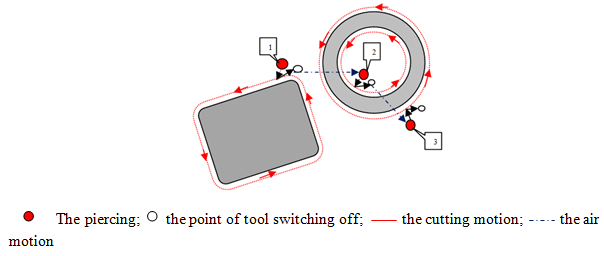
\includegraphics[width=0.9\textwidth]{elements.png}
  \caption{Cutting scheme example of two parts using standard cutting technique}
  \label{elements}
  \end{center}
\end{figure}

The objective function
(cutting cost $F_{cost}$)
is calculated by \cite{ru04}:
\begin{equation}
F_{cost} =
L_{on} \cdot C_{on} +
L_{off} \cdot C_{off} +
N_{pt} \cdot C_{pt}
\to \min
\label{cost}
\end{equation}

$L_{off}$ is length of air tool path;
$L_{on}$ is length of working tool path;
$C_{off}$ is cost of air tool path unit;
$C_{on}$ is cost of working tool path unit;
$N_{pt}$ is numbers of piercing;
$C_{pt}$ is cost of one piercing.

In general when using different types ($j = \overline{1, k}$) of piercing
the $F_{cost}$ is calculated by:

\begin{equation}
  F_{cost} =
  L_{on} \cdot C_{on} +
  L_{off} \cdot C_{off} +
  \sum_{j=1}^k L_{pt}^j \cdot C_{pt}^j
  \to \min
  \label{cost-n}
\end{equation}

The problem of cost function minimization is considered as
\textit{generalized travelling salesman problem (GTSP) with restrictions}
\cite{ru04,ru05}.
The formalization of minimization problem of cutting time and cost
for CNC sheet cutting machines is presented in \cite{ru04}.

In \cite{Dewil2016Nov,Hoeft1997Sep,Petunin2015Nov}
the following classes of cutting tool routing problems
for CNC sheet cutting machines are allocated:

\begin{itemize}

\item The Traveling Salesman Problem – TSP;

\item The Generalized Traveling Salesman Problem – GTSP;

\item The Continuous Cutting Problem – CCP;

\item The End Point Cutting Problem – ECP;

\item Intermittent Cutting Problem – ICP;

\item Based on conception of contours cutting by segment \cite{Petunin2015Nov}
the new class of optimization tool routing problem is presented:
Segment Continuous Cutting Problem (SCCP).

\end{itemize}

The detailed analysis of existing methods,
which are solving the optimization problem
of cutting tool route, was presented in \cite{Dewil2016Nov}.
A few algorithms of tool routing for other technological equipments
are particularly described in \cite{Grotschel,Ghiani}.
In these articles there are questions relating to
cutting time optimization.
The present methods of cutting time optimization
relate to minimization of idle moves time and
slightly to minimization of cutting time.
The analysis of current methods is provided below.

Analysis  of existing methods of cost function minimizing showed that
airtime and length of air motion are usually minimized
during cutting path optimizing.
The following researchers present algorithms for idle moves optimization.
Yang et al. \cite{Yang2010}
describe the airtime optimization problem in leather cutting.
They proposed the hybrid intelligence algorithm.
Castelino et al. \cite{d2003tool}
describe an algorithm for airtime minimizing
by optimally connecting the tool path.
They consider heuristic methods
that are used in order to obtain the optimal or near optimal solutions.
Murzakaev et al \cite{ru17}
consider problem of idle moves length minimization.
The model is presented for standard cutting technique.
In order to minimize cutter idle moves length
the three metaheuristics
(Simulated Annealing, Threshold Accepting, Great Deluge Algorithm)
were chosen.
They propose the generalized scheme of problem solving.
The algorithm of idle moves minimizing is proposed by Chen et al \cite{Chen2014Dec}.
They divide into two sub-optimal problems
(pattern cutting order and entry/exit cutting point)
and solve ones using an ant colony optimization algorithm
(min-max ant system).
Lee and Kwon \cite{Lee2006Dec}
consider tool path problem and
proposed two-step genetic algorithm.
The aim is to minimize the idle moving of cutting tool.
They combine global search for piercing optimization
and local search for part sequencing.
The two stage of sequential optimization procedure for
nesting and cutting sequence are presented by Sherif et al \cite{Sherif2014Oct}.
The objectives are maximizing the material utilization
and minimizing the cutter idle moves.
They consider simulated annealing algorithm
in order to find the near optimal cutting tool path.

Analysis of existing methods shows
the deficiency of research in the field of piercing numbers $N_{pt}$
reducing
and length of cutting tool motion  $L_{on}$
in solving the optimization problem (\ref{cost-n}).
In \cite{Manber1984Jan}
authors consider the problem of $N_{pt}$ reducing
in thermal cutting of sheet material in terms of graph theory.
It should be noted that the precedence constrain was not taken into account
and the intersection of the existing cuts is allowed.
The problem of cutting path optimization in terms of cutting of parts group
with one of pierce point is considered in \cite{ru22}.
The last stage of solving the problem
(cutter routing optimization at idle moves)
is reduced to the TSP.
The problem of cutter routing optimization at CNC machines
is formulated and the mathematical model of total cutting time minimization
is proposed by using standard and special cutting techniques
by Faizrahmanov et al. \cite{ru23}.
Verhoturov et al. \cite{ru24}
present ``chained'' cutting technique in order to
minimize the numbers of pierce points.

The one of cutting time and cost minimization methods is
application of special cutting techniques.
In order to optimize the cutting parameters
and to observe the necessary cutting requirements
the some special cutting techniques are used.
There are ``chained'' cutting \cite{ru28},
common cut \cite{ru25}, partial cutting of contour
with the subsequent completion of the contour cutting
after cutting the contour of another part, et al.
Petunin and Krotov \cite{ru25} proposed the
classification of various cutting techniques
used to form the cutting tool path.
The cutting techniques are classified into three main classes:
standard cutting, multi-contour cutting and multi-segment cutting technique.
Every contour is cut with pierce point by using
\textit{standard cutting technique}.
The numbers of pierce points equal numbers of contours.
The several contours are cut in one cutting segment
with one pierce point by using
\textit{multi-contour cutting technique}.
For example, the multi-contour cutting includes ``chained'' cutting, common cut.
The several cutting segments are cut with several pierce points by using
\textit{multi-segment technique}.

Analysis of optimization problem solutions shows that
there are no or are negligible considered the questions
about cutting cost optimization in addressed articles.
To this end the methodology of exact calculation of
cutting cost objective function is conducted in this article.
In optimization problem (\ref{cost-n})
there are difficulties in calculating the basic parameters
$C_{on}, C_{off}, C_{pt}$
depending on many factors in order to exact computation of
$F_{cost}$
and construct the exact optimal cutting path.
For CNC laser cutting machines
$C_{on}, C_{off}, C_{pt}$
depend on the type of laser used in CNC machine,
type and thickness of treatment material.
The selected factors depend on analytically or tabular functions.
The formulas of
$C_{on}, C_{off}, C_{pt}$
calculation and their values may significantly differ
for various CNC sheet cutting machines.
The analysis of existing methods for cutting cost calculation
shown the insufficiency of research in the field.
The time per pierce in laser cutting process is calculated in
\cite{ru06}.
In \cite{ru07}
the laser cutting cost is compared with water jet,
plasma and oxygen cutting costs
when treatment sheet material of 1.0114
(thicknesses $\Delta=3-10 mm$).
In \cite{ru08}
the assessment of plasma and $CO_2$
laser cutting machines operating cost is performed.
But it should be noted that
the calculation of cost parameters
remains outside the scope of present researches,
hence the calculation of
$C_{on}, C_{off}, C_{pt}$
values and consequently exact calculation of cost function
$F_{cost}$
value are actual problems today,
which are solved in this article.
The methodology of cost parameters calculation in objective function
$F_{cost}$
is developed.

As seen from (\ref{cost-n})
$F_{cost}$
also depends on
$L_{on}, L_{off}$ and $N_{pt}$,
in turn $L_{on}$ depends on value of working tool speed $V_{on}$.
The value of $V_{on}$ is usually constant parameter
which is programming during the NC program development,
but as the practical shows \cite{ru09,Tavaeva2015Nov}
the value of actual working speed of cutting tool
is varied by various technological factors and parameters of NC programs.
Consequently problem of accurate calculation of cost function (\ref{cost-n})
in optimization problem of tool path routing is arisen.
In order to solve the encountered problem
the need of correction parameters calculation for $V_{on}$
values is emerged.
It should be noted that
the question of exact calculation of  $V_{on}$ values remains open,
then there is a need of research in order to calculate the correction parameters of  $V_{on}$
values and consequently cutting cost in this article for CNC laser cutting machines.

It is observed that $L_{on}, L_{off}$ and $N_{pt}$
are interdependent.
In some cases the reduction of  $N_{pt}$
leads to some increase of total cutting tool path length value $L_{on}$
due to cutting motion between contours.
Wherein the length of air path $L_{off}$ is reduced.

The problem of cost function minimization (\ref{cost-n})
during treatment of figured parts from sheet material
at CNC cutting machines is solved by the optimization of parameters
$L_{on}, L_{off}$ and $N_{pt}$.
As the practice shows the length of cutting tool motion  $L_{on}$
and numbers of pierce points $N_{pt}$
have the greatest impact on the cutting cost compared with the length of air tool motion $L_{off}$.
Depending on the thickness and type of material the $C_{pt}$
can reach up to 33\% from $C_{on}$
and at the same time can exceed the $C_{off}$
by three orders \cite{ru14}.
Consequently the most interest are the methods of solving the problem aimed at the minimizing
$L_{on}$ and $N_{pt}$.

The article is organized as follows.
The model of $F_{cost}$
calculation and basic parameters
$C_{on}, C_{off}, C_{pt}$
is presented in Section 2.1.
Exact calculation of $V_{on}$
values and values of correction coefficients for $V_{on}$
is given in Section 2.2.
Based on the exact computation of objective functions
the cutting path and cutting cost are evaluated as a true.
The results of the computational experiment are presented in Section 3.

\section{Exact calculation of cost function $F_{cost}$ in the cutter path optimization problem}

\subsection{Model of basic cost parameters $C_{on}, C_{off}, C_{pt}$ calculation}

The most important economic characteristic of the developed NC program quality is the cost $F_{cost}$
of cutting parts at CNC machine.
$F_{cost}$ includes the costs of electricity and expendable materials,
maintenance of a CNC machine and other operating costs incurred during cutting.
The problem of exact calculation of cost function $F_{cost}$
in optimizing of cutting tool route related with search of adequate value  $F_{cost}$,
which calculation depends on basic parameters $C_{on}, C_{off}, C_{pt}$.
The allotted parameters in turn depend on values of
$L_{on}, L_{off}$ and $N_{pt}$.
The functional dependence
$C_{on}, C_{off}, C_{pt}$
on type and thickness of material,
laser type in CNC machine,
cost of expendable materials,
cost of laser and technological gases,
depreciation of equipment
can be set either table functions or analytically.
Frequently the cutting cost is not often considered in blank production
or is calculated based on normative is not dependent on values of
$C_{on}, C_{off}, C_{pt}$.
Obviously that necessity of cutting cost calculation
arises on manufacturer which provides
cutting material service for the third-party firm.
As a rule during cutting cost calculation only
$L_{on}$
is taken into account
which usually equals compound perimeter of cutting parts edge contours
that leads to inaccurate cutting cost calculation.
Subsequently the calculation methodology of cutting cost parameters
is actual problem today.

The calculation methodology of
cutting cost parameters
in optimization problem of cutting path applied to CNC laser cutting machine
(laser type is $CO_2$)
is considered.
In order to calculate $C_{on}$
the following notations for cost parameters calculation on 1 m of cutting tool motion are entered:
$C_{exp.mat}$ - the cost of expendable materials
(for example, adjudge, protective glass, gas tubes);
$C_{tech}$  - the cost of technological gas
(nitrogen or oxygen depending on processed material);
$C_{las}$ - the cost of cutting gas
(when working on a gas flow laser);
$C^{on}_{elec}$ - the cost of electricity;
$C^{on}_{salary}$ - the cost related with salary of accompanying personnel;
$C^{on}_A$ - amortization of equipment.
In general
$C_{on}$
is calculated by:

\begin{equation}
C_{on} =
C^{on}_{elec} + C_{tech} + C_{las} + C_{exp.mat} + C^{on}_{salary} + C^{on}_A
\label{eq1.3}
\end{equation}

In order to calculate
$C^{on}_{elec}, C_{tech}, C_{las}, C_{exp.mat}, C^{on}_{salary}, C^{on}_A$
the additional notations are entered:
$t_{on}$  - the time spent on 1 m of cutting tool motion, h.;
$P_{on}$  - the electricity costs for 1 hour of CNC laser machine work on cutting motion, $kW/h$;
$V_{tech}$  - technological gas consumption, $m^3/h$ ;
$V_{las}$ - laser gas consumption, $m^3/h$;
$C_{elec}$  - electricity cost per 1 kW;
$C_{las M^3}$  - the cost of 1 $m^3$ laser gas;
$C_{tech M^3}$  - the cost of 1 $m^3$ technological gas;
$C_{exp.mat.Unit}$  - the cost of expendable materials unit;
$t_{exp.mat.Term}$  - serviceable life of expendable materials;
$C_{salary}$ - cost of 1 h work of accompanying personnel;
$A$ – amortization of 1 h work of CNC laser cutting machine;
$N$ - useful life of equipment;
$C_{equip}$  - initial cost of the CNC laser cutting machine.

$C^{on}_{elec}, C_{tech}, C_{las}, C_{exp.mat}, C^{on}_{salary}, C^{on}_A$
are calculated by:

\begin{equation}
\label{eq1.4}
C^{on}_{elec} = P_{on} t_{on} C_{elec}
\end{equation}

\begin{equation}
  \label{eq1.5}
  C_{tech} = V_{tech} C_{tech M^3} t_{on}
\end{equation}

\begin{equation}
  \label{eq1.6}
  C_{las} = V_{las} C_{las M^3} t_{on}
\end{equation}

\begin{equation}
  \label{eq1.7}
  C_{exp.mat} = \frac{C_{exp.mat.Unit} t_{on}}{t_{exp.mat.Term}}
\end{equation}

\begin{equation}
  \label{eq1.8}
  C^{on}_{salary} = C_{salary} t_{on}
\end{equation}

\begin{equation}
  \label{eq1.9}
  C^{on}_A = \frac{1}N \frac{C_{equip}}{1920} t_{on}
\end{equation}

In order to calculate $C_{off}$
the following notations are entered:
$P_{off}$ – the electricity costs for 1 hour of CNC laser machine work on air motion, $kW/h$;
$t_{off}$ – the time spent on 1 m of air tool motion, h.
Consequently
$C_{off}$
is calculated by:

\begin{equation}
  \label{eq1.10}
  C_{off}
  = P_{off} t_{off} C_{elec}
  + C_{salary} t_{off}
  + \frac{1}N \frac{C_{equip}}{1920} t_{off}
\end{equation}

In order to calculate $C_{pt}$
the following notations for cost parameters calculation on 1 pierce point are entered:
$C^{pt}_{exp.mat}$ - the cost of expendable materials
(for example, adjudge, protective glass, gas tubes);
$C^{pt}_{tech}$ - the cost of technological gas
(nitrogen or oxygen depending on processed material);
$C^{pt}_{las}$ - the cost of cutting gas
(when working on a gas flow laser);
$C^{pt}_{elec}$ - the cost of electricity;
$C^{pt}_{salary}$ - the cost related with salary of accompanying personnel;
$C^{pt}_A$ - amortization of equipment.
In general
$C_{pt}$
is calculated by:

\begin{equation}
  \label{eq1.11}
  C_{pt}
  = C^{pt}_{elec}
  + C^{pt}_{exp.mat}
  + C^{pt}_{las}
  + C^{pt}_{tech}
  + C^{pt}_{salary}
  + C^{pt}_A
\end{equation}

In order to calculate
$C^{pt}_{elec}, C^{pt}_{exp.mat}, C^{pt}_{las}, C^{pt}_{tech}, C^{pt}_{salary}, C^{pt}_A$
the additional notations are entered:
$P_{pt}$ – the electricity costs for 1 pierce point, $kW/h$;
$t_{pt}$  – the time spent on 1 pierce point, h.
Consequently
$C^{pt}_{elec}, C^{pt}_{exp.mat}, C^{pt}_{las}, C^{pt}_{tech}, C^{pt}_{salary}, C^{pt}_A$
are calculated by:

\begin{equation}
  \label{eq1.12}
  C^{pt}_{elec} = P_{pt} t_{pt} C_{elec}
\end{equation}

\begin{equation}
  \label{eq1.13}
  C^{pt}_{exp.mat} = V_{tech} C_{tech M^3} t_{pt}
\end{equation}

\begin{equation}
  \label{eq1.14}
  C^{pt}_{las} = V_{las} C_{las M^3} t_{pt}
\end{equation}

\begin{equation}
  \label{eq1.15}
  C^{pt}_{exp.mat} = \frac{C_{exp.mat.Unit} t_{pt}}{t_{exp.mat.Term}}
\end{equation}

\begin{equation}
  \label{eq1.16}
  C^{pt}_{salary} = C_{salary} t_{pt}
\end{equation}

\begin{equation}
  \label{eq1.17}
  C^{pt}_A = \frac{1}N \frac{C_{equip}}{1920} t_{pt}
\end{equation}

During calculation of $C_{pt}$
and $C_{on}$
the following parameters $C^{pt}_{las}$
and $C_{las}$ must be taken into account
when processing of material at flow-through gas laser machines.
The parameter $C^{pt}_{tech}$
must be considered during calculation of $F_{cost}$
when technological gas is applied.

Consequently,
$F_{cost}$
can be written as follows:

\begin{multline}
  \label{eq1.18}
  F_{cost}
  = L_{on} \Big(
    C^{on}_{elec} + C_{tech} + C_{las} + C_{exp.mat} + C^{on}_{salary} + C^{on}_A
    \Big)
  + L_{off} C_{off} \\
  + N_{pt} \Big(
    C^{pt}_{elec} + C^{pt}_{exp.mat} + C^{pt}_{las} + C^{pt}_{tech} + C^{pt}_{salary} + C^{pt}_A
    \Big)
\end{multline}

The main expendable materials for gas laser include:
swivel mirrors, focusing lenses, protective glasses, nozzles, adjusting units, gas tubes.
The main expendable materials for fiber laser are nozzles, protective glasses, focusing lenses.
And for the case of using solid-state lasers,
the expendable materials are
optical pumping lamps, protective glasses, mirrors, a quantron, an active element.
In \cite{ru14} the values of cost parameters
$C_{on}, C_{off}, C_{pt}$
are presented by taken into account the above parameters
(\ref{eq1.3})-(\ref{eq1.17})
for CNC laser cutting machine by example ByStar 3015.
For each type of material the parameters
$C_{on}, C_{off}, C_{pt}$
are calculated by taken into account that
$V_{on}=const$.
As the practical shown \cite{ru09,Tavaeva2015Nov}
the value of actual working speed of cutting tool
is varied by various technological factors and parameters of NC programs.
Consequently problem of accurate calculation of cost function (\ref{cost-n})
in optimization problem of tool path construction is arisen.
In order to solve the encountered problem
the need of correction parameters calculation for $V_{on}$
values is emerged.

\begin{figure}
  \begin{center}
  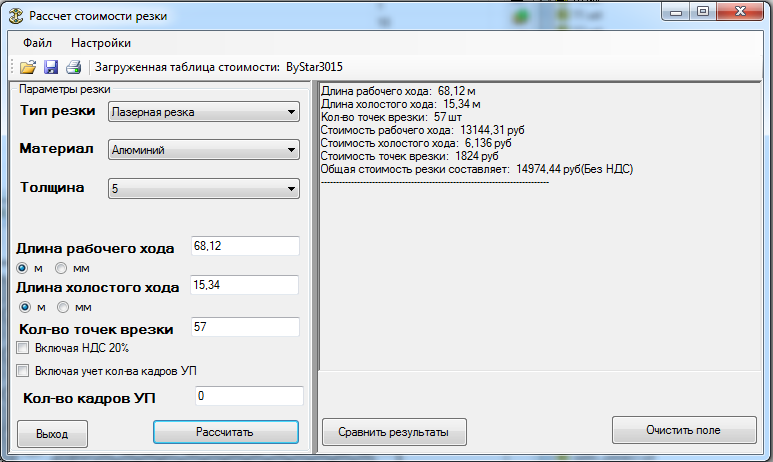
\includegraphics[width=0.9\textwidth]{app.png}
  \caption{The interface of ``Cutting cost calculation'' subsystem}
  \label{app-window}
  \end{center}
\end{figure}

Based on proposed methodology
the subsystem ``Cutting cost calculation''
was developed by using Net. Framework technology.
A subsystem may be integrated with existing CAM software.
Fig. \ref{app-window}
presents interface of developed subsystem.
In order to calculate
$F_{cost}$
the values of basic cost parameters
$C_{on}, C_{off}, C_{pt}$
are added into database in XML format.

\subsection{Accurate calculation of $V_{on}$ in objective function from the example of the CNC laser cutting machine ByStar 3015}

The inaccuracy of the actual cutting time and cost calculation is due to the fact that $V_{on}$,
which is programmed as constant value in NC program,
is actually varied by various technological factors.
It was found that increasing of frames numbers in NC program
for various sets of parts,
which have the same total perimeter of the contours,
the actual $V_{on}$ is decreased \cite{ru09,Tavaeva2015Nov}.
The reasons why NC program can contain a large numbers of frames
is mainly due to the contours of complex geometry (for example, splines)
when converting from CAD systems to a CAM
are divided into a large numbers of geometric primitives
due to the difference of geometric file formats
(for example, on segments of straight lines and circular arcs),
i.e. approximated by simple geometric primitives.
The difference in formats is due to the fact that
almost all CNC systems are equipped with only linear and circular interpolators.
As a rule the approximation of a complex geometry reduces to a linear approximation.

The functional dependence of $V_{on}$
should be determined by science-based table functions or analytically.
However in practice
$V_{on}=const$
and in this case the accuracy of objective function calculation
during cutting path optimization is not provided
The algorithmization of objective function (\ref{cost-n})
calculation based on science–based determination of function parameters
is requirement for the development of cutting tool path optimization algorithms.
The cutting tool route is optimal only if
the objective function is adequate calculated.
For this reason the exact parameters values of objective function (\ref{cost-n})
must be calculated.

Some practical results on determining
dependence of cutting speed on number of NC program commands
are given below.
Based on received results the objective function (\ref{cost-n})
can exactly calculated and exact optimal cutting path can constructed.

The research was conducted for following materials:
1.0114 (thickness $\Delta=1-10$ mm) and
AWAIMg3 (thickness $\Delta=1-5$ mm).
In order to conduct experiments the 150 NC programs
for cutting of various types of parts with numbers of frames
$n=\overline{10, 5000}(n \in \mathbb{N})$
for 1.0114
and 150 NC programs for cutting of various types of parts with numbers of frames
$n = \overline{10, 2000} (n \in \mathbb N)$
for AWAIMg3
were developed.

The statistical materials were processed by using ``Mathcad''.
Based on received results the following upshots were made:

\begin{enumerate}
\item
The actual average speed of cutting tool speed $V_{act}$
is monotonically decreasing function depending on frames numbers of NC program
(Fig. \ref{plot});

\item
The predetermined cutting tool speed $V_{on}$
coincides with the actual average speed
when the numbers of frames reaches a certain threshold value $N$.
When the frames numbers $n < N$,
then the actual speed is greater than predetermined cutting tool speed,
if the frames numbers of NC program is arisen ($n>N$)
then the actual speed is less than
predetermined cutting tool speed of NC program
(in the experiments the reduction of average actual cutting tool speed value
compared with predetermined cutting tool speed in NC program is 70\%);

\item
The threshold value $N$ is varied for different thickness and grade of material.
\end{enumerate}

\begin{figure}
  \begin{center}
  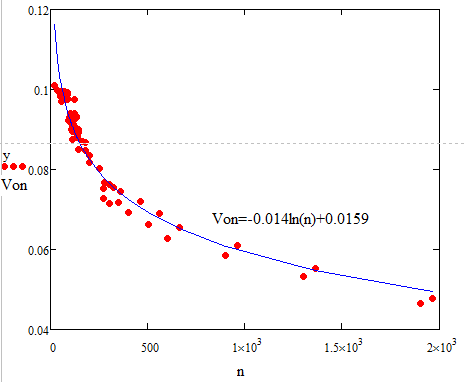
\includegraphics[width=0.8\textwidth]{plot.png}
  \caption{Change of the real cutting tool speed for AWAIMg3, $\Delta=1$ mm}
  \label{plot}
  \end{center}
\end{figure}

In order to present the results of computational experiments
the following notations are introduced:
$n$ – number of NC program commands;
$V_{act}$ - the actual speed of cutting tool;
$N$ – the number of commands when ;
$\sum \varepsilon_n^2$ - the deviation squares sum of the original data
from the values of the approximation functions at these points.

When approximation the actual speed dependence
presented on point chart on the number of commands
with approximating curves in ``Mathcad''
$\sum \varepsilon_n^2 \to 0$
for all values of studied grade materials
and thickness are achieved using logarithmic approximation function.
Fig. \ref{plot}
presents following results for material of AWAIMg3 with $\Delta=1 mm$.
Similar results were obtained for AWAIMg3 with $\Delta=1-5 mm$
and 1.0114 with $\Delta=1-10 mm$.
The generalized formulas for calculating of
cutting tool speed by example CNC laser cutting machine
ByStar3015 are presented in table \ref{formulas-table}.

\begin{table}
  \begin{tabular}{c | c | c }
  Material & $\Delta$ &  Formulas for cutting tool speed calculation \\
  \hline \hline
  1.0114 & 1 mm & $V_{on}=-0.025 \cdot \ln n + 0.25$ \\
  1.0114 & 2 mm & $V_{on}=-0.015 \cdot \ln n + 0.1711$ \\
  1.0114 & 3 mm & $V_{on}=-0.009 \cdot \ln n + 0.1062$ \\
  1.0114 & 3.5 mm & $V_{on}=-0.006 \cdot \ln n + 0.0759$ \\
  1.0114 & 4 mm & $V_{on}=-0.006 \cdot \ln n + 0.0709$ \\
  1.0114 & 8 mm & $V_{on}=-0.003 \cdot \ln n + 0.0443$ \\
  1.0114 & 10 mm & $V_{on}=-0.002 \cdot \ln n + 0.0359$ \\
  AWAIMg3 & 1 mm & $V_{on}=-0.014 \cdot \ln n + 0.1589$ \\
  AWAIMg3 & 2 mm & $V_{on}=-0.004 \cdot \ln n + 0.0641$ \\
  AWAIMg3 & 3 mm & $V_{on}=-0.001 \cdot \ln n + 0.0315$ \\
  AWAIMg3 & 5 mm & $V_{on}=-7 \cdot 10^{-4} \cdot \ln n + 0.0182$ \\
  \hline
  \end{tabular}
  \caption{Generalized table of formulas for calculating of cutting tool speed by example CNC laser cutting machine ByStar3015}
  \label{formulas-table}
\end{table}

For subsystem ``Cutting cost calculation''
the module,
in which the complexity of processed contours
and consequently developed functional dependences
(presented in table \ref{formulas-table})
may be taken into account,
was developed.
This enable to exact calculate an objective function
$F_{cost}$.
Based on practice obtained results of
$F_{cost}$
calculation considering developed formulas
the values of cutting cost is significantly differ
compared with values of
$F_{cost}$
calculated with above developed methodology.

\begin{figure}
  \centering
  \subfigure[Standard cutting technique]{
    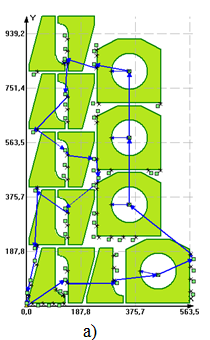
\includegraphics[width=0.3\textwidth]{path-a.png}
    \label{path-const}
  }
  \subfigure[Special cutting technique]{
    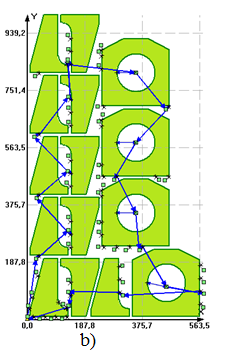
\includegraphics[width=0.32\textwidth]{path-b.png}
    \label{path-var}
  }
  \caption{Optimal cutting path }
  \label{optimal-paths}
\end{figure}

In turn application of developed formulas
during nesting and cutting path construction
leads to modification of cutting path.
The obtained path is accurate
compared with path constrained with
$V_{on}=const$.
For example,
fig. \ref{optimal-paths}
presents the cutting path optimization
for nesting of 15 parts
(material of AWAIMg3, $\Delta=1 mm$).
Each contour is cut used standard cutting technique
(when number of piercing equals number of parts contours).
In order to reduce acceptable solutions set
the acceptable piercings set is limited with finite aggregate consists of 55 points
(these points are green squares in fig. \ref{optimal-paths},
in turn points of tool switching off are X).
The blue arrows are idle moves of cutter.
The number of NC program commands for this nesting is
$n=120$.
For the case of fig. \ref{path-const}
$V_{on}=const=0.1 m/s$,
for the case of fig. \ref{path-var}
$V_{on}=-0.014 \cdot \ln n + 0.1589$.

Based on proposed results (fig. \ref{optimal-paths})
the accurate calculation of objective function ensures
not only the exact computation of function extremum value
but also the correct results of optimal cutting path search
taking into account parts complexity.

\section{Computational experiments}

The proposed methodology of
$F_{cost}$
calculation taking into account dependence of cutting speed
$V_{on}$
on parts complexity is useful during
practice technological problems solving
in terms of optimal cutting route planning on CNC thermal machines.
There is example of cutting route planning below with reduction of
$F_{cost}$
for shaped parts taken into account
application of special cutting techniques
with thermal deformation reduction developed in \cite{ru26}.
The conditions of thermal deformation reduction
during nesting and cutting route planning are considered in \cite{ru01}.

Based on algorithms presented on \cite{ru26}
the cutting tool route for nesting is automatically built at CAD/CAM ``SIRIUS''.
In order to evaluate the the effectiveness of developed special cutting techniques
two nestings are obtained by using standard (Fig. \ref{cut-std})
and special (Fig. \ref{cut-spec})
cutting techniques for various types of parts.

Fig. \ref{cut-std} presents the cutting tool path
built for various geometrical types of parts including circles using standard cutting techniques.
Fig. \ref{cut-spec} presents the cutting tool path built for various geometrical types of parts
including circles using special cutting techniques.

\begin{figure}
  \centering
  \subfigure[Standard cutting technique]{
    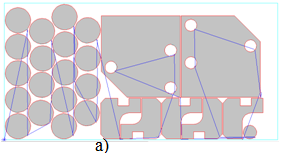
\includegraphics[width=0.47\textwidth]{path-std.png}
    \label{cut-std}
  }
  \subfigure[Special cutting technique]{
    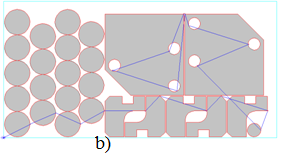
\includegraphics[width=0.47\textwidth]{path-spec.png}
    \label{cut-spec}
  }
  \caption{Cutting scheme example}
  \label{cutting}
\end{figure}

Table \ref{f-cost}
presents computational results of basic cutting parameters and values of $F_{cost}$
for obtained NC programs.
The calculation of $F_{cost}$
was carried out by using ``Cutting cost calculation''.
The results are calculated for AWAIMg3 $\Delta = 1$ and 5 mm.

\begin{table}
  \begin{tabular}{c | c | c | c | r r r | c | r r | r}
  Material & $\Delta$ & Technique & Fig. & $N_{pt}$ & $L_{off}, m$ & $L_{on}, m$ & $n$ & $F_{cost}, rub$ & $F^n_{cost}, rub$ & \% \\
  \hline \hline
  \multirow{4}{*}{AWAIMg3} & \multirow{2}{*}{1 mm} & Standard & Fig. \ref{cut-std}     & 32  & 16.43   & 36.82 & \multirow{4}{*}{130} & 809.5 & 866.5 & 6.6 \\
                         &                    & Special  & Fig. \ref{cut-spec} & 18  & 8.6  & 36.97 &                      & 757.1 & 814.3 & 7 \\
                         & \multirow{2}{*}{5 mm} & Standard & Fig. \ref{cut-std}  & 32 & 16.43 & 36.82 &                    & 13121.1 & 16062.2 & 18.3 \\
                         &                    & Special  & Fig. \ref{cut-spec}  & 18 & 8.6 & 36.97 &                      & 12748.1 & 15701.2 & 18.8 \\
  \hline
  \end{tabular}
  \caption{Results of $F_{cost}$ calculation}
  \label{f-cost}
\end{table}

The following notations in table \ref{f-cost}
are used:
$n$ – numbers of frames in NC program;
$F_{cost}$ - the cutting cost calculated taking into account that $V_{on}=const$;
$F^n_{cost}$ - the cutting cost calculated taking into account that $V_{on}=var$
and depends on the frames numbers of NC program;
\% - value of difference between
$F_{cost}$
and
$F^n_{cost}$.

The results presented in Table \ref{f-cost} indicate that
the basis cutting parameters are reduced by using special cutting techniques
compared with standard cutting.
In turn the difference between
$F_{cost}$
and
$F^n_{cost}$.
reaches to 18\%.

\section{Conclusion}

In this paper the following results were obtained:

\begin{enumerate}

\item
In order to exact calculate objective function and consequently
to construct exact tool path the methodology of objective function
$F_{cost}$
and basic cost parameters calculation
is presented for CNC laser cutting machines.
Due to the problem of exact
$F_{cost}$
values calculation have arisen on many production factories
and based on proposed methodology the subsystem
``Cutting cost calculation''
were developed used Net. Framework technology,
which may be integrated with existing CAM software;

\item
The functional dependencies on number of NC program commands for
$V_{on}$
are developed.
These dependencies ensure exact calculation
of objective function
$F_{cost}$
and exact tool optimization path construction.
For subsystem ``Cutting cost calculation''
the module of exact cutting cost computation
of cutting cost was developed used functional dependencies for
$V_{on}$;

\item
In order to evaluate the developed results
the computational experiments have been conducted
taking into account previously proposed
special cutting techniques compared with standard cutting.
The cutting route is constructed
with taking into account the thermal deformation reduction.
The correct
$F_{cost}$
values calculation is carried out
with developed above methodology given the
$V_{on} = var(F_{cost}^n)$
and
$V_{on} = const(F_{cost})$.
The results shown that
the cutting cost is reduced by using special cutting techniques
compared with standard cutting.
In turn the difference between
$F_{cost}$.
and
$F_{cost}^n$
reaches to 18\%.

\end{enumerate}

\section{Acknowledgments}
The work was supported by the Russian Foundation for Basic Research
(grant \textnumero 19-01-00573).

\bibliographystyle{splncs04}
\bibliography{tavaeva}
% \nocite{*}

\end{document}
